\usetikzlibrary{arrows.meta, shapes.geometric, positioning, calc}

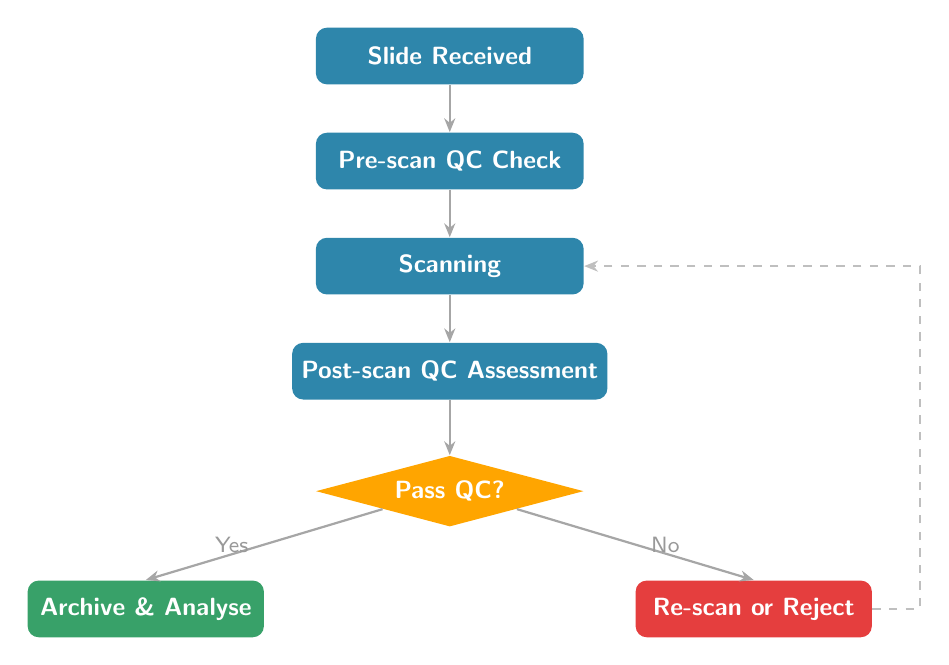
\begin{tikzpicture}[
    node distance = 0.6cm,
    every node/.style = {font=\small\sffamily},
    proc/.style = {
        rectangle, rounded corners=4pt,
        fill={rgb,255:red,46;green,134;blue,171},
        text=white, minimum width=3.4cm, minimum height=0.72cm,
        align=center, font=\small\sffamily\bfseries
    },
    decision/.style = {
        diamond, aspect=2.6,
        fill={rgb,255:red,255;green,165;blue,0},
        text=white, minimum width=3.4cm, minimum height=0.9cm,
        align=center, font=\small\sffamily\bfseries,
        inner sep=1pt
    },
    pass/.style = {
        rectangle, rounded corners=4pt,
        fill={rgb,255:red,56;green,161;blue,105},
        text=white, minimum width=3.0cm, minimum height=0.72cm,
        align=center, font=\small\sffamily\bfseries
    },
    fail/.style = {
        rectangle, rounded corners=4pt,
        fill={rgb,255:red,229;green,62;blue,62},
        text=white, minimum width=3.0cm, minimum height=0.72cm,
        align=center, font=\small\sffamily\bfseries
    },
    arr/.style = {
        -{Stealth[length=5pt,width=4pt]},
        line width=0.8pt, color=gray!70
    },
    lbl/.style = {font=\footnotesize\sffamily, text=gray!80}
]

%% Main vertical chain
\node[proc]     (recv)     {Slide Received};
\node[proc,     below=0.6cm of recv]     (prescan)  {Pre-scan QC Check};
\node[proc,     below=0.6cm of prescan]  (scan)     {Scanning};
\node[proc,     below=0.6cm of scan]     (postscan) {Post-scan QC Assessment};
\node[decision, below=0.7cm of postscan] (decide)   {Pass QC?};

%% Outcome nodes
\node[pass, below left=0.9cm and 1.5cm of decide]  (archive) {Archive \& Analyse};
\node[fail, below right=0.9cm and 1.5cm of decide] (rescan)  {Re-scan or Reject};

%% Arrows — main chain
\draw[arr] (recv)     -- (prescan);
\draw[arr] (prescan)  -- (scan);
\draw[arr] (scan)     -- (postscan);
\draw[arr] (postscan) -- (decide);

%% Arrows — decision branches
\draw[arr] (decide.south west) -- (archive.north)
    node[lbl, midway, left=2pt] {Yes};
\draw[arr] (decide.south east) -- (rescan.north)
    node[lbl, midway, right=2pt] {No};

%% Loop-back dashed arrow for Re-scan
\draw[arr, dashed, color=gray!50]
    (rescan.east) -- ++(0.6,0) |- (scan.east);

\end{tikzpicture}
